
\section{Supplementary figures}
\begin{figure}[htbp!]
\center
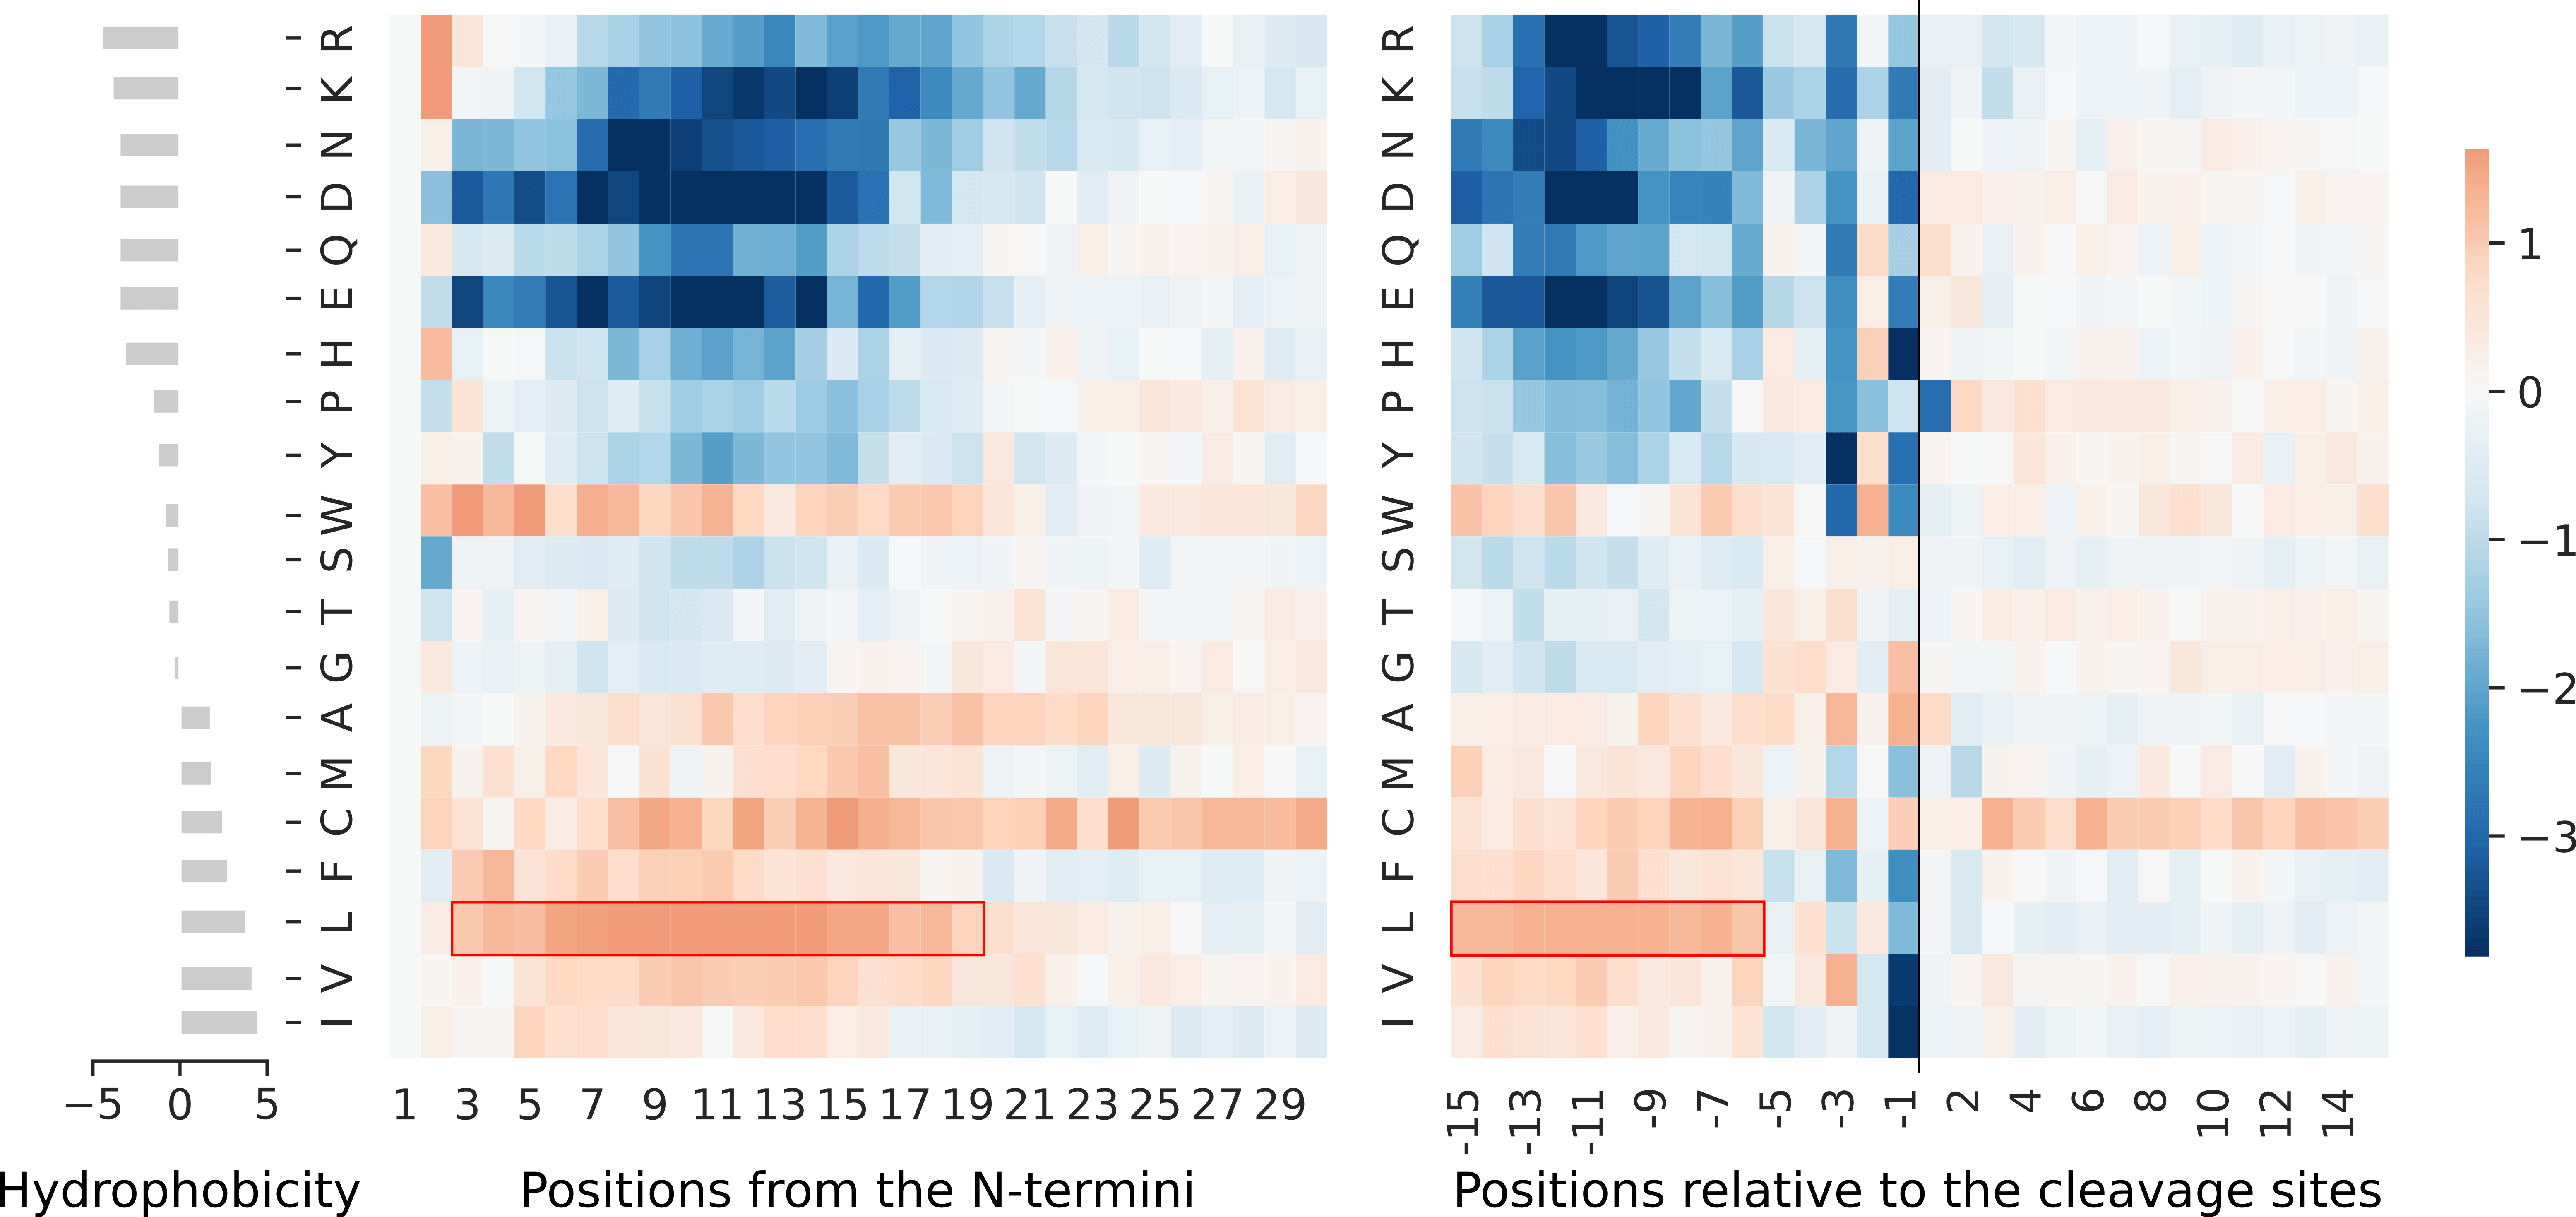
\includegraphics[width=1\textwidth]{appendix/Razor/Figs/figS1_bitscore_heatmap.png}
\caption[Signal peptides (SPs) show a strong hydrophobic property (1,964 experimentally validated SPs, 13,237 non-SPs).]{\textbf{ Signal peptides (SPs) show a strong hydrophobic property (1,964 experimentally validated SPs, 13,237 non-SPs). }  The bar plot shows Kyte and Doolittle’s hydrophobicity scale. The heatmaps show the enrichment of residues in bit scores by aligning SPs from the N-termini (left) and at the cleavage sites (right, black vertical line). The (-3, -1) rule for the cleavage site motif is shown (left). The unfilled, red rectangles indicate the enrichment of leucine residues (L).
}%the List of Figures because of the *}
\label{fig:appendix_razor_S1}
\end{figure}


\begin{figure}[htbp!]
\center
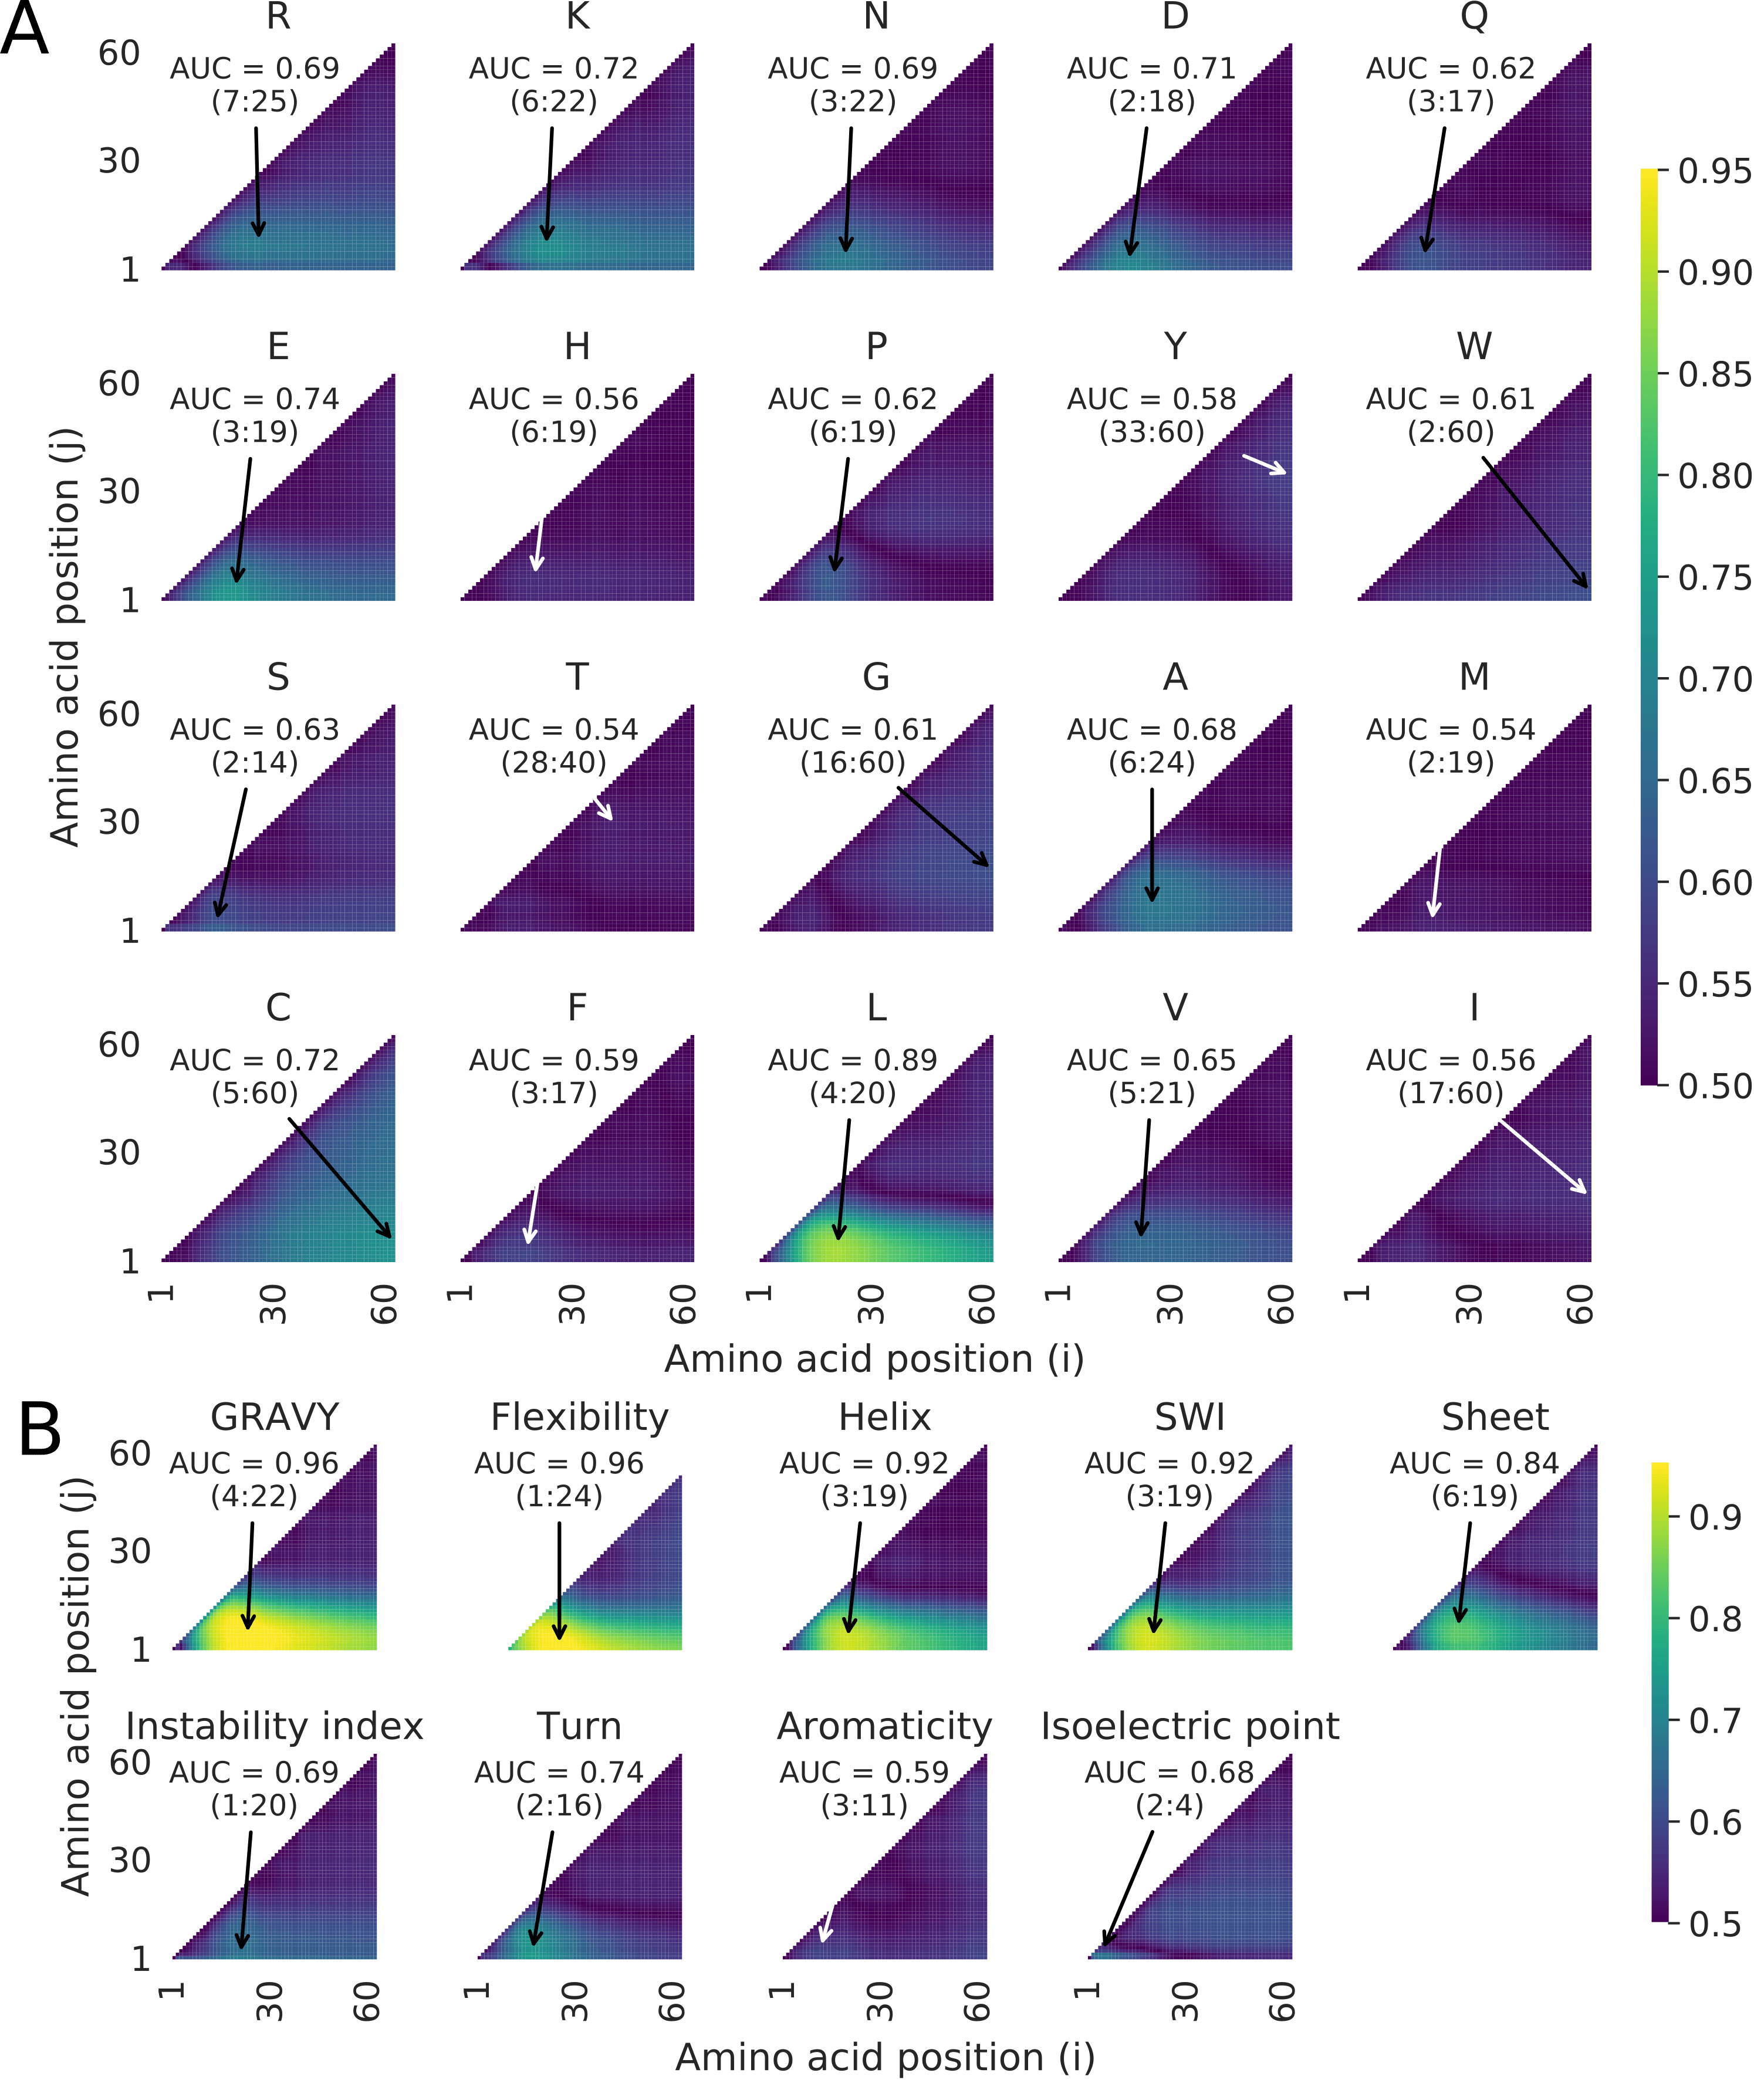
\includegraphics[width=1\textwidth]{appendix/Razor/Figs/AUC_matrix_Eukaryota.png}
\caption[Leucine (L) composition within the N-terminal region 4:20 shows the highest AUC score in classifying the presence or absence of eukaryotic signal peptides (1,964 and 13,237, respectively).]{\textbf{ Leucine (L) composition within the N-terminal region 4:20 shows the highest AUC score in classifying the presence or absence of eukaryotic signal peptides (1,964 and 13,237, respectively).} Amino acid compositions were calculated from positions i to j. \textbf{(A)} AUC heatmaps for all residues. \textbf{(B)} GRAVY, Flexibility, Helix and SWI are the top four features ranked by AUC scores. AUC, Area Under the Curve; GRAVY, GRAnd average of hydropathicitY; SWI, Solubility-Weighted Index. 

}%the List of Figures because of the *}
\label{fig:appendix_razor_S2}
\end{figure}


\begin{figure}[htbp!]
\center
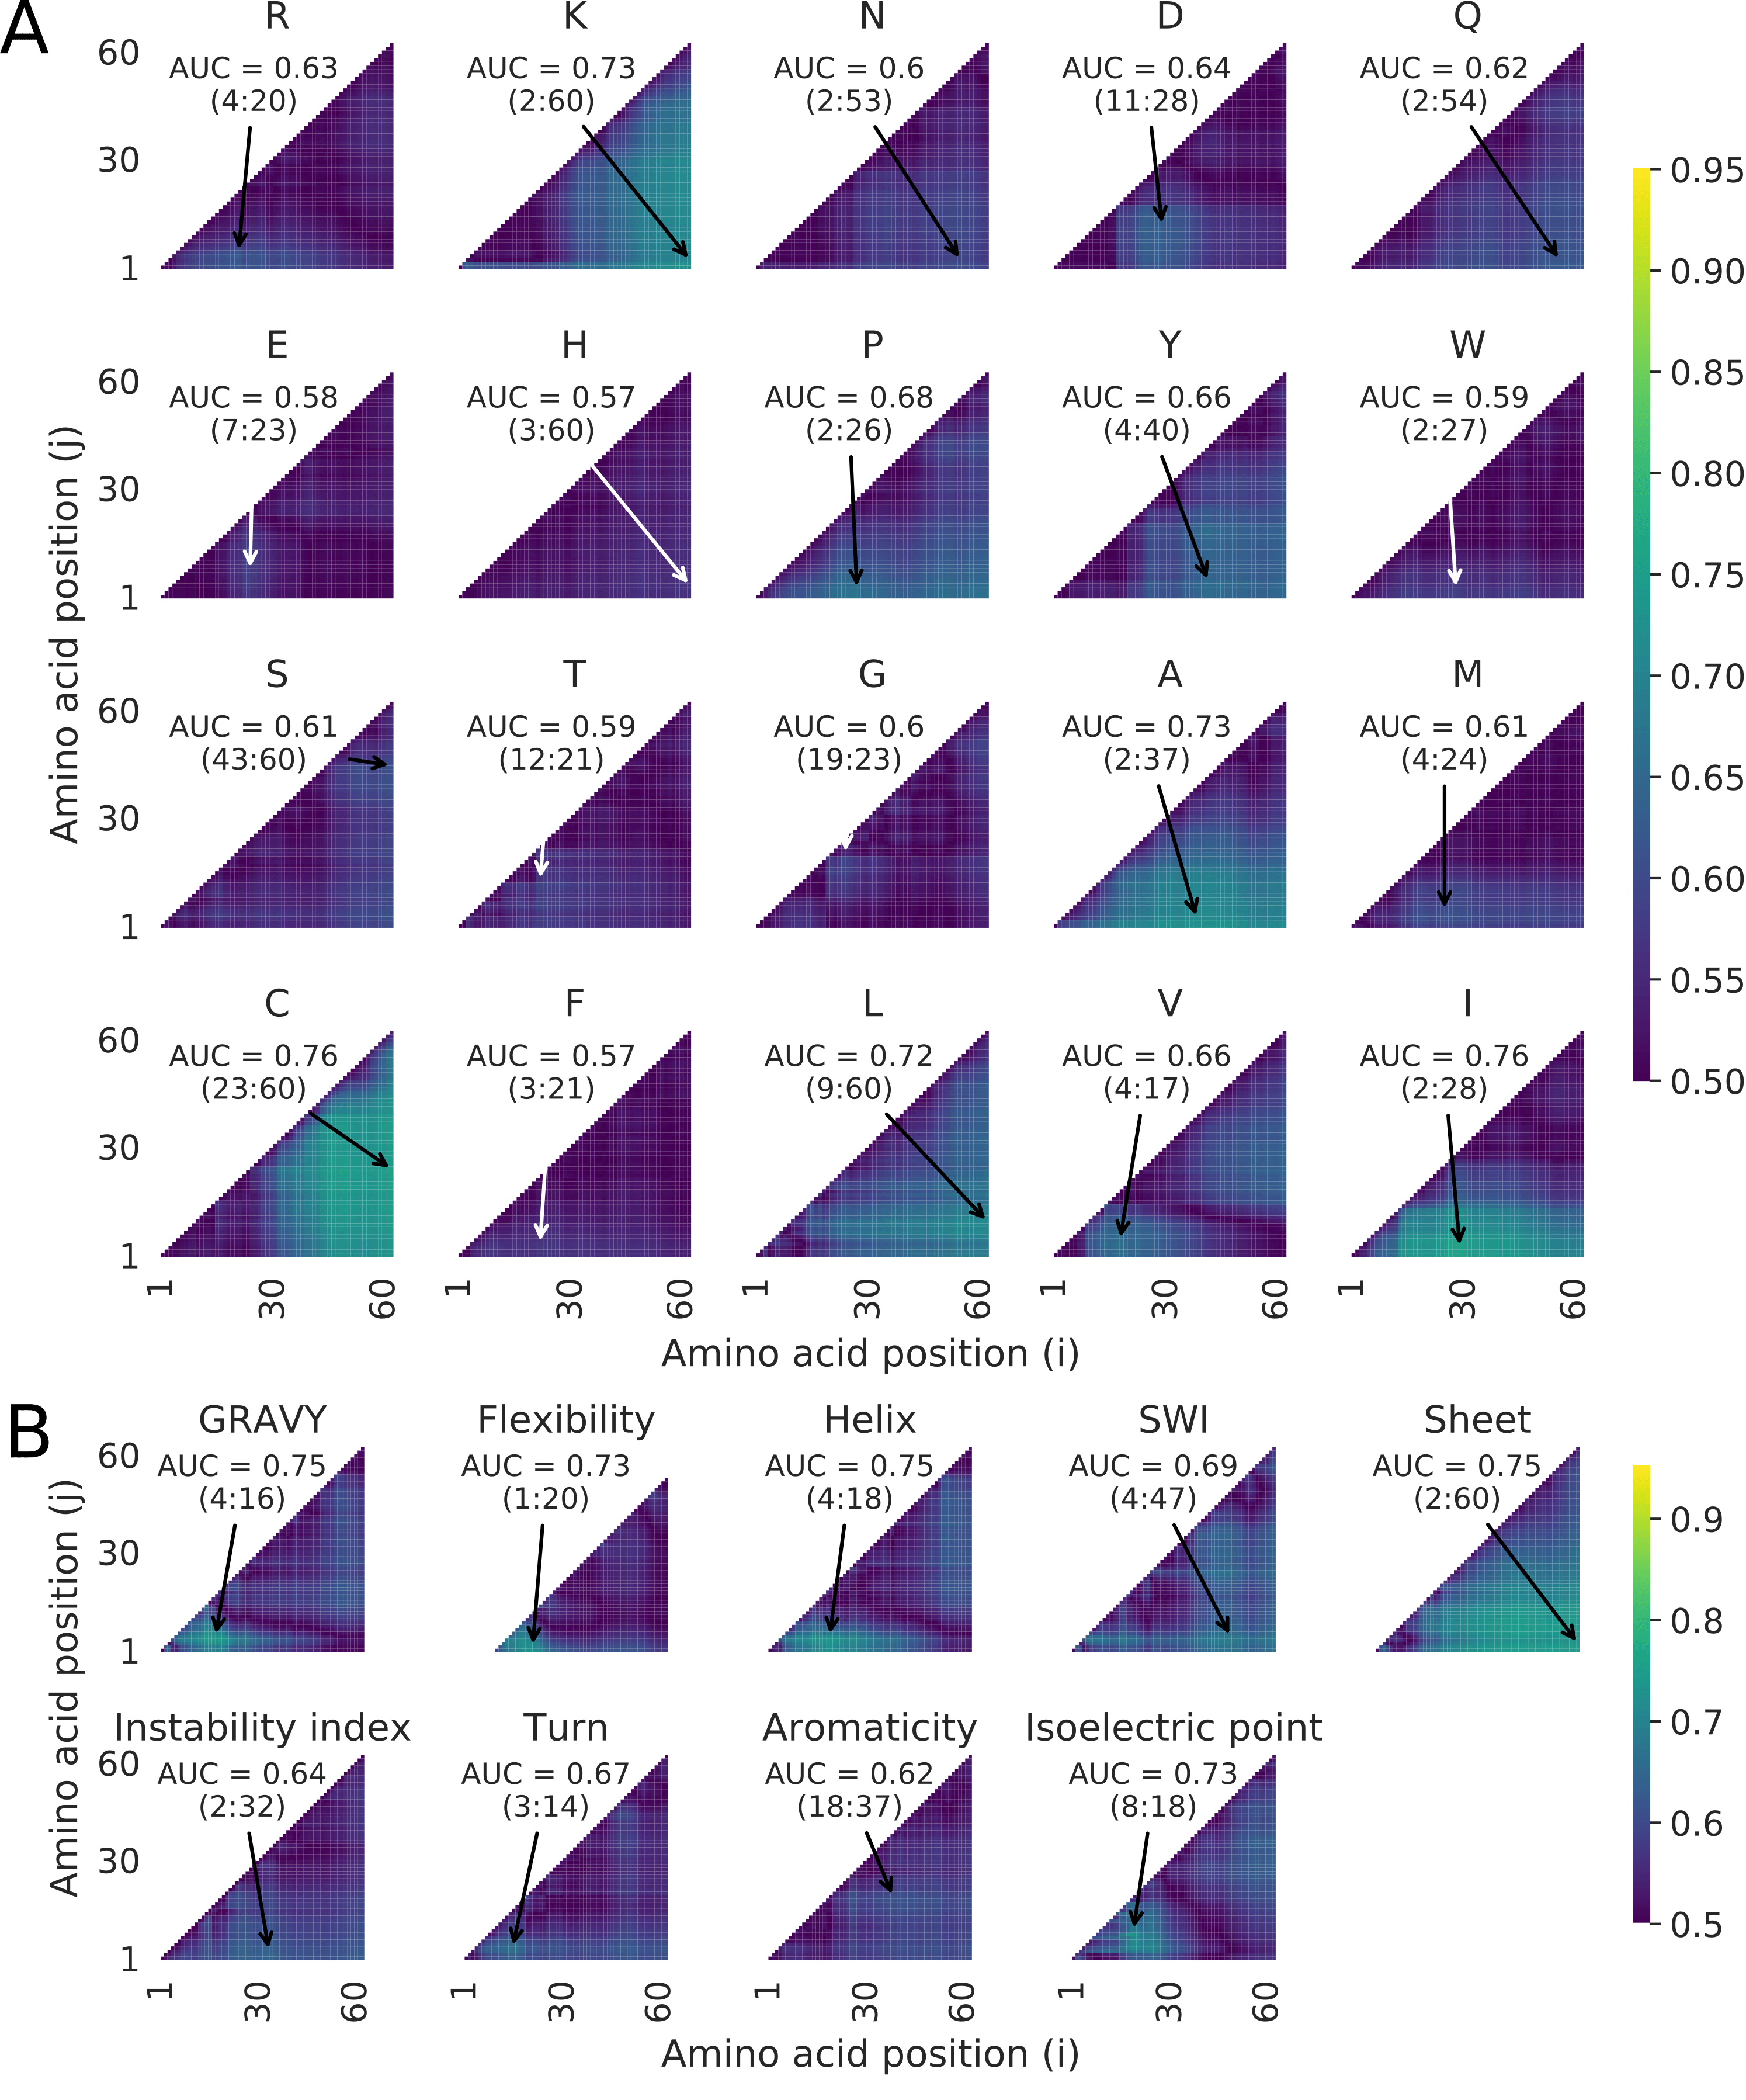
\includegraphics[width=1\textwidth]{appendix/Razor/Figs/AUC_matrix_Toxins.png}
\caption[Isoleucine (I) composition within the N-terminal region 2:28 shows the highest AUC score in classifying toxin and non-toxin SPs (261 and 1,738, respectively).]{\textbf{Isoleucine (I) composition within the N-terminal region 2:28 shows the highest AUC score in classifying toxin and non-toxin SPs (261 and 1,738, respectively).}  Amino acid compositions were calculated from positions i to j. \textbf{(A)} AUC heatmaps for all residues. Cysteine shows a higher AUC score at the mature region (23:60) as many toxins are cysteine-rich. \textbf{(B)} GRAVY, Flexibility, Helix, SWI, Isoelectric point are the top features ranked by AUC scores. Although Sheet has a high AUC score, the region 2:60 extends beyond the normal SP length of around 30 residues. AUC, Area Under the Curve; GRAVY, GRAnd average of hydropathicitY; SWI, Solubility-Weighted Index.


}%the List of Figures because of the *}
\label{fig:appendix_razor_S3}
\end{figure}

\begin{figure}[htbp!]
\center
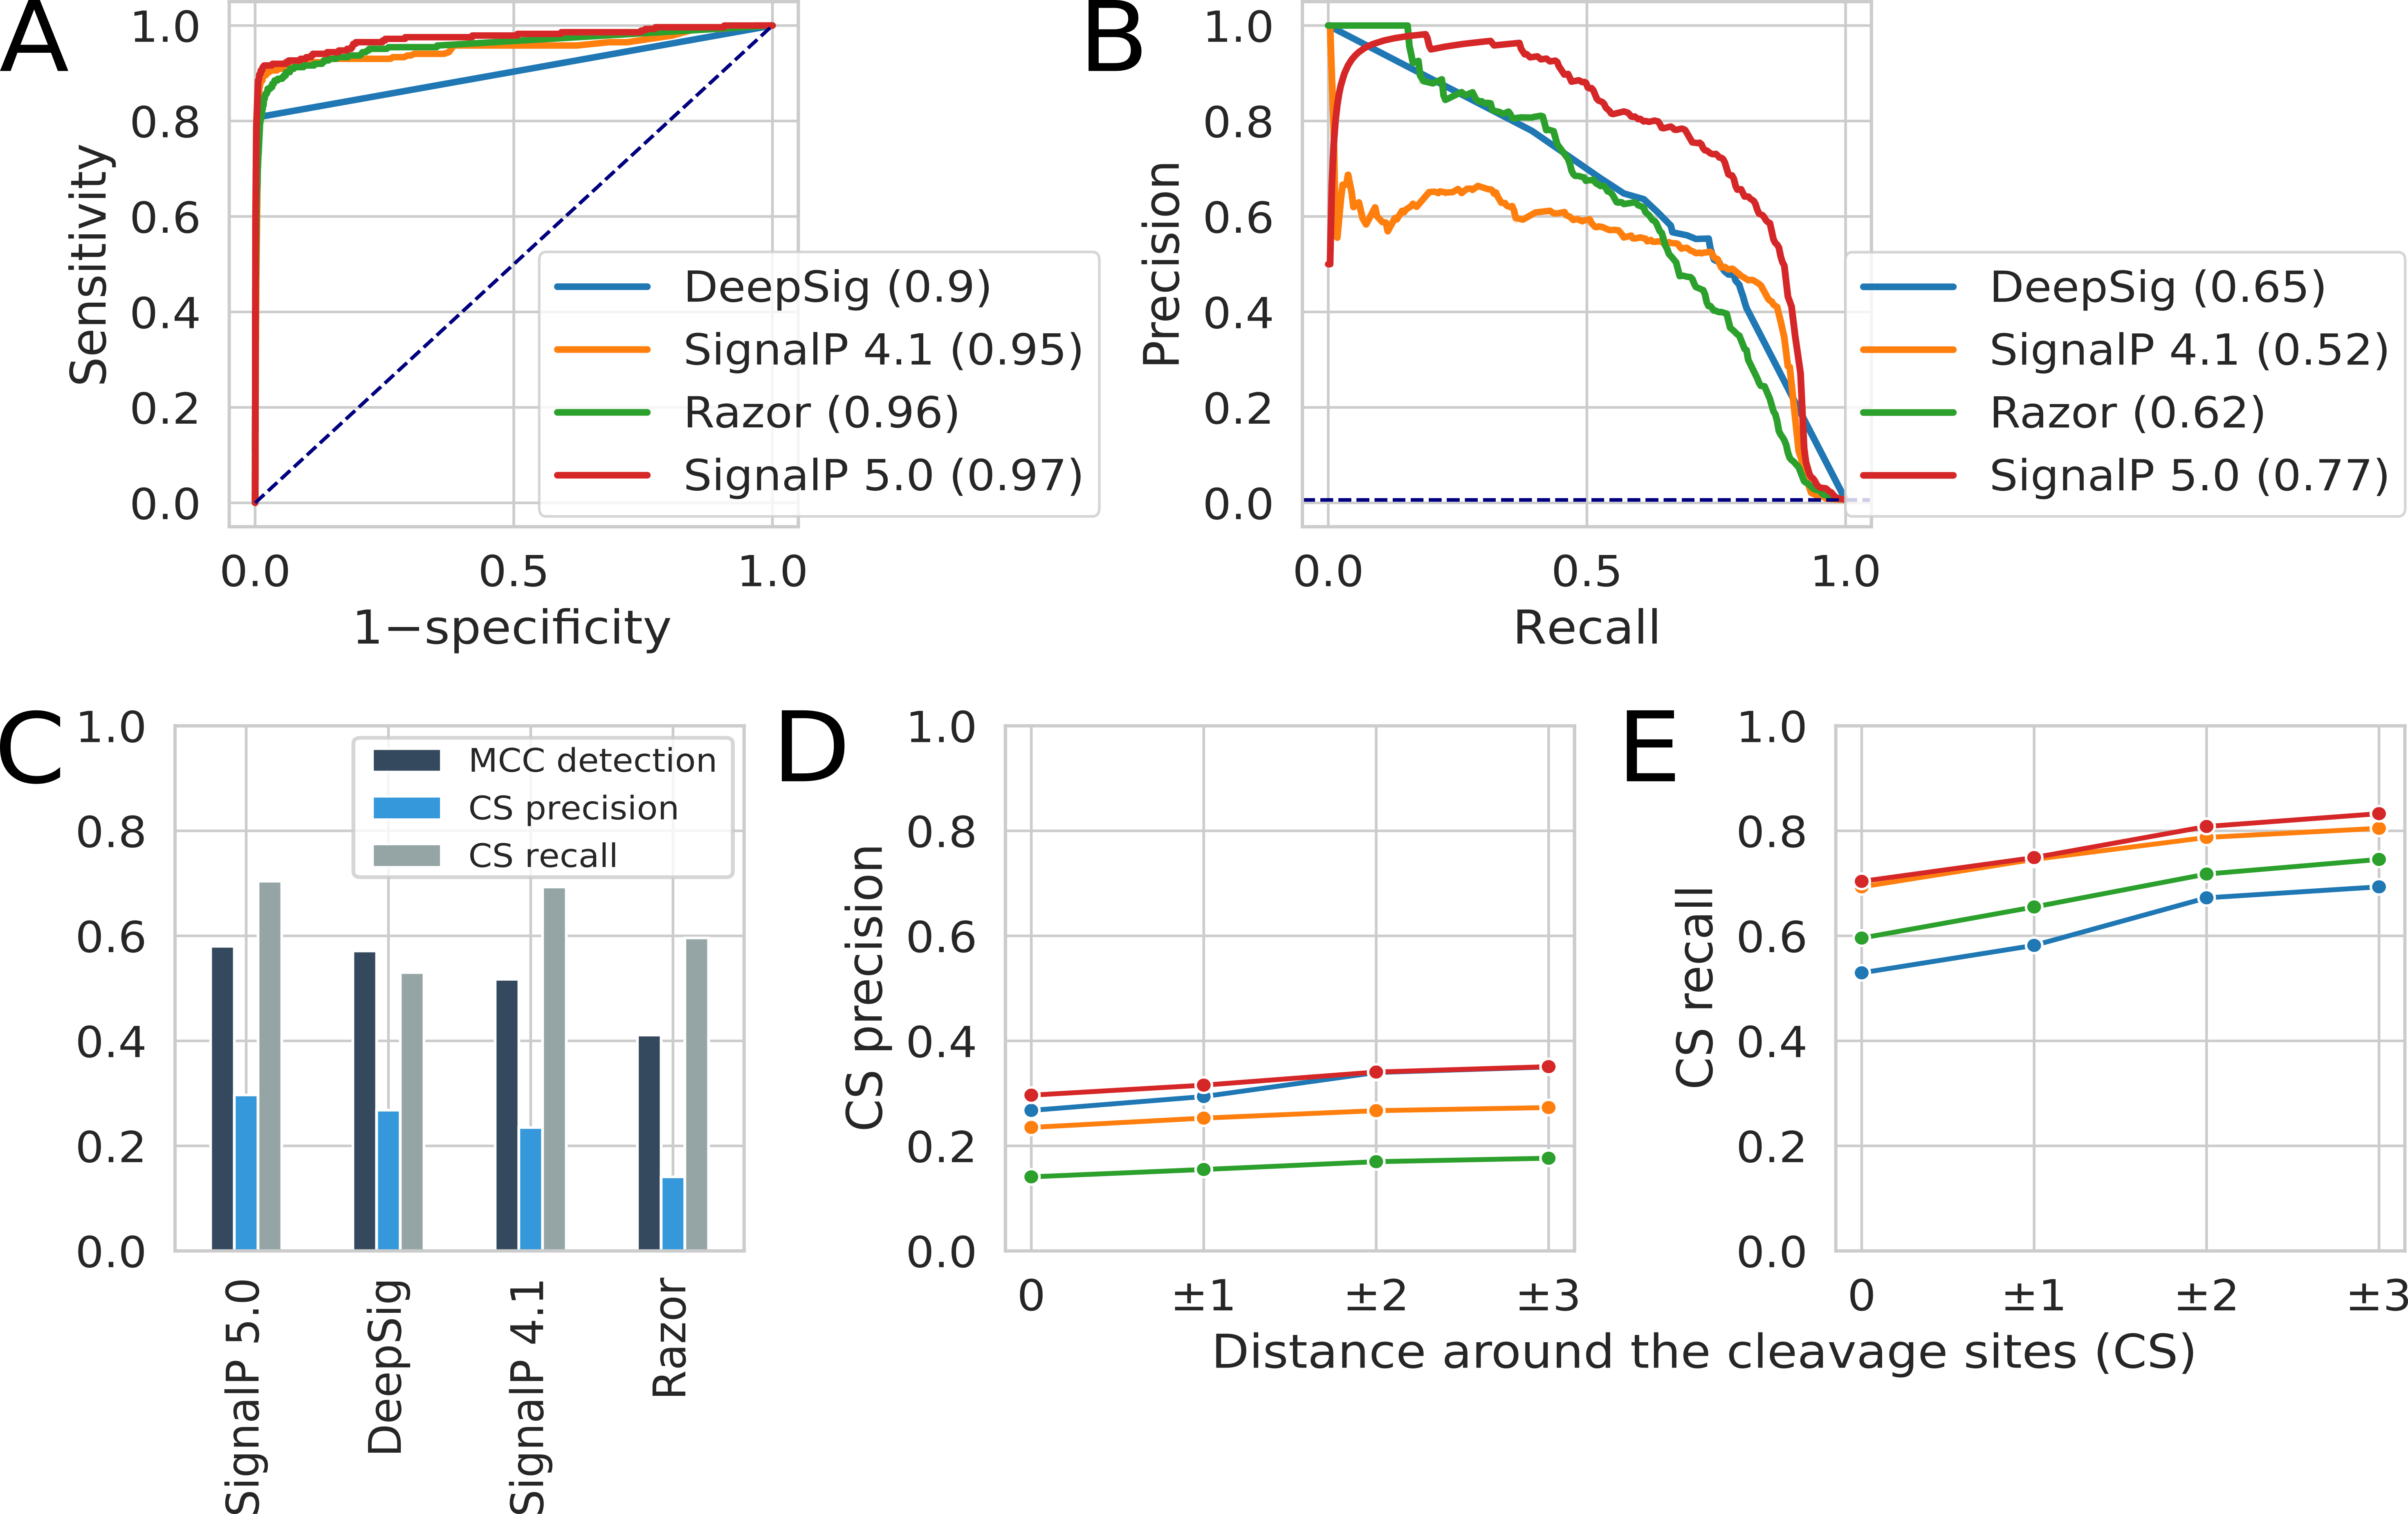
\includegraphics[width=1\textwidth]{appendix/Razor/Figs/figS4_new_benchmarking_cleavage_sites_all.png}
\caption[Performance of Razor and state-of-the-art in predicting eukaryotic SPs using an independent test set (SPs=241, non-SPs=52,055).]{\textbf{Performance of Razor and state-of-the-art in predicting eukaryotic SPs using an independent test set (SPs=241, non-SPs=52,055).}  Receiver operating characteristic curves \textbf{(A)} and precision recall curves \textbf{(B)} of the SP prediction tools. Areas under the curves are shown in parentheses. The dotted lines show the performance of a random classifier. \textbf{(C)} Matthew’s Correlation Coefficients (MCC) of the SP prediction tools. The cleavage site (CS) precisions \textbf{(D)} and recalls \textbf{(E)} of windows surrounding the cleavage sites are shown. Data are available in Supplementary Tables S3 and S4.

}%the List of Figures because of the *}
\label{fig:appendix_razor_S4}
\end{figure}

\clearpage

\begin{figure}[htbp!]
\center
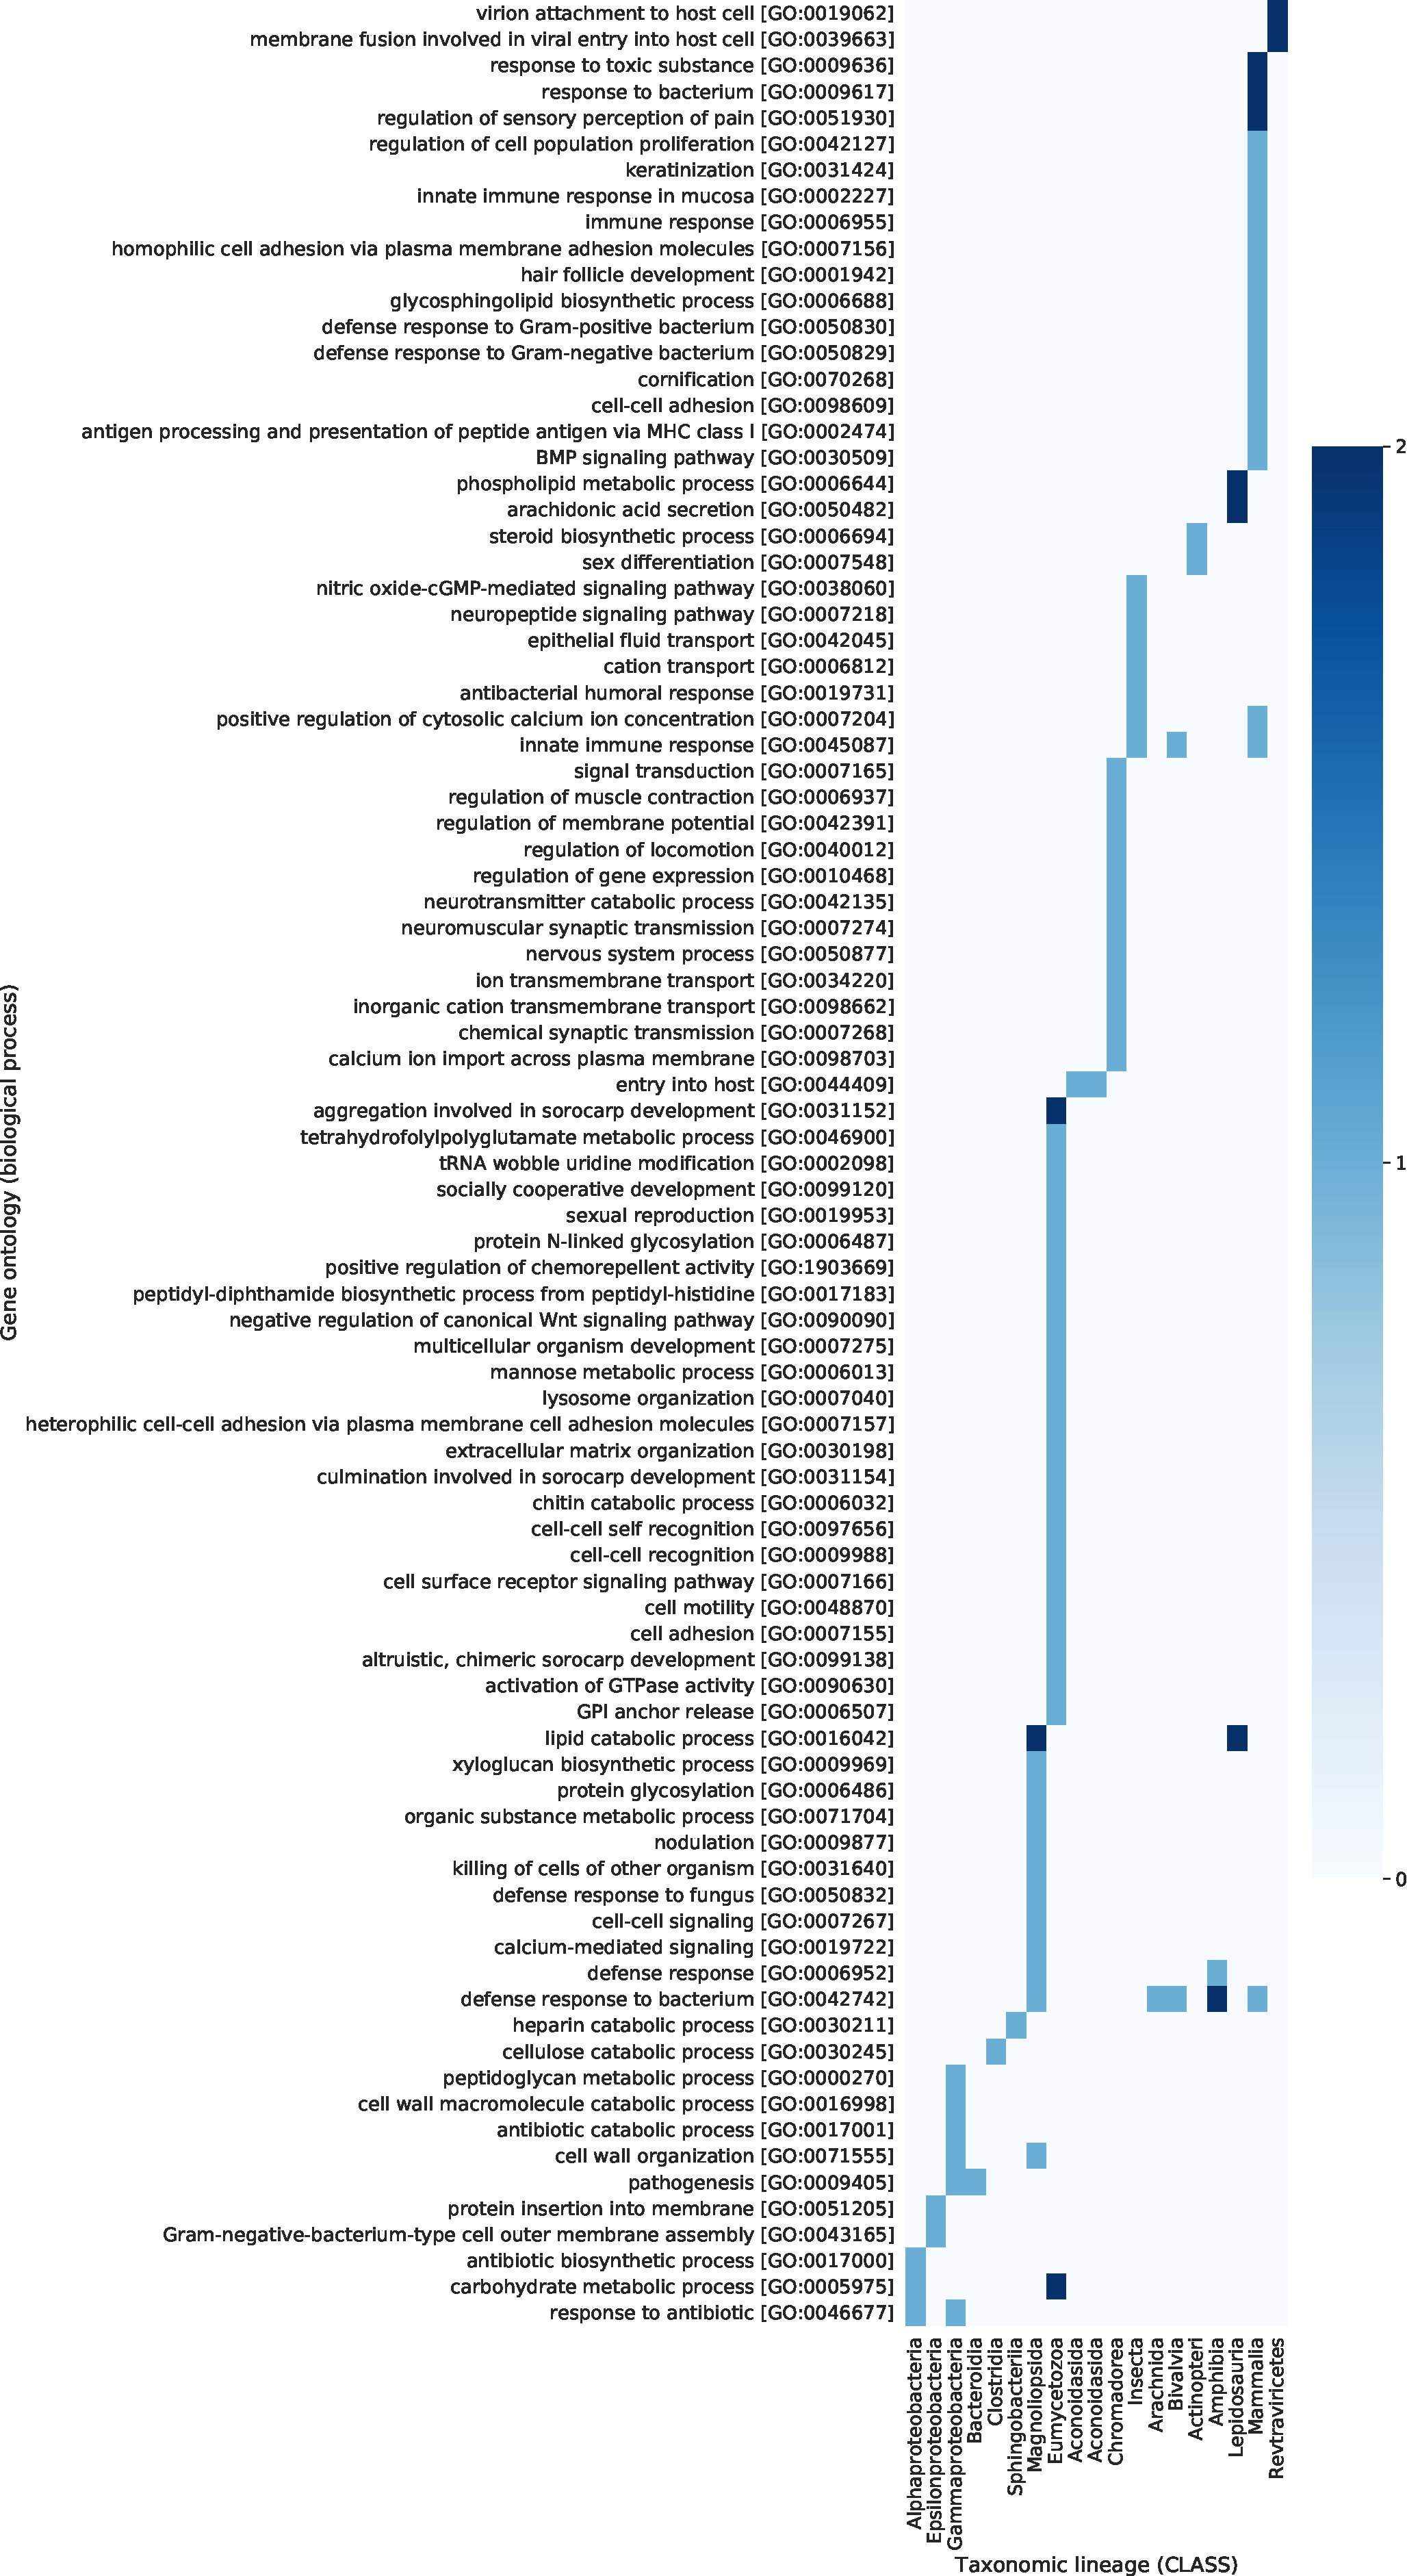
\includegraphics[width=0.75\textwidth]{appendix/Razor/Figs/toxins_GO_biological_process.pdf}
\caption[Gene ontology (GO) annotations (biological process) for the predicted toxin SPs.]{\textbf{Gene ontology (GO) annotations (biological process) for the predicted toxin SPs.} A total of 54 out of 100 predicted sequences had GO terms. The scale bar indicates the frequencies of GO terms for the predicted sequences.

}%the List of Figures because of the *}
\label{fig:appendix_razor_S5}
\end{figure}

\begin{figure}[htbp!]
\center
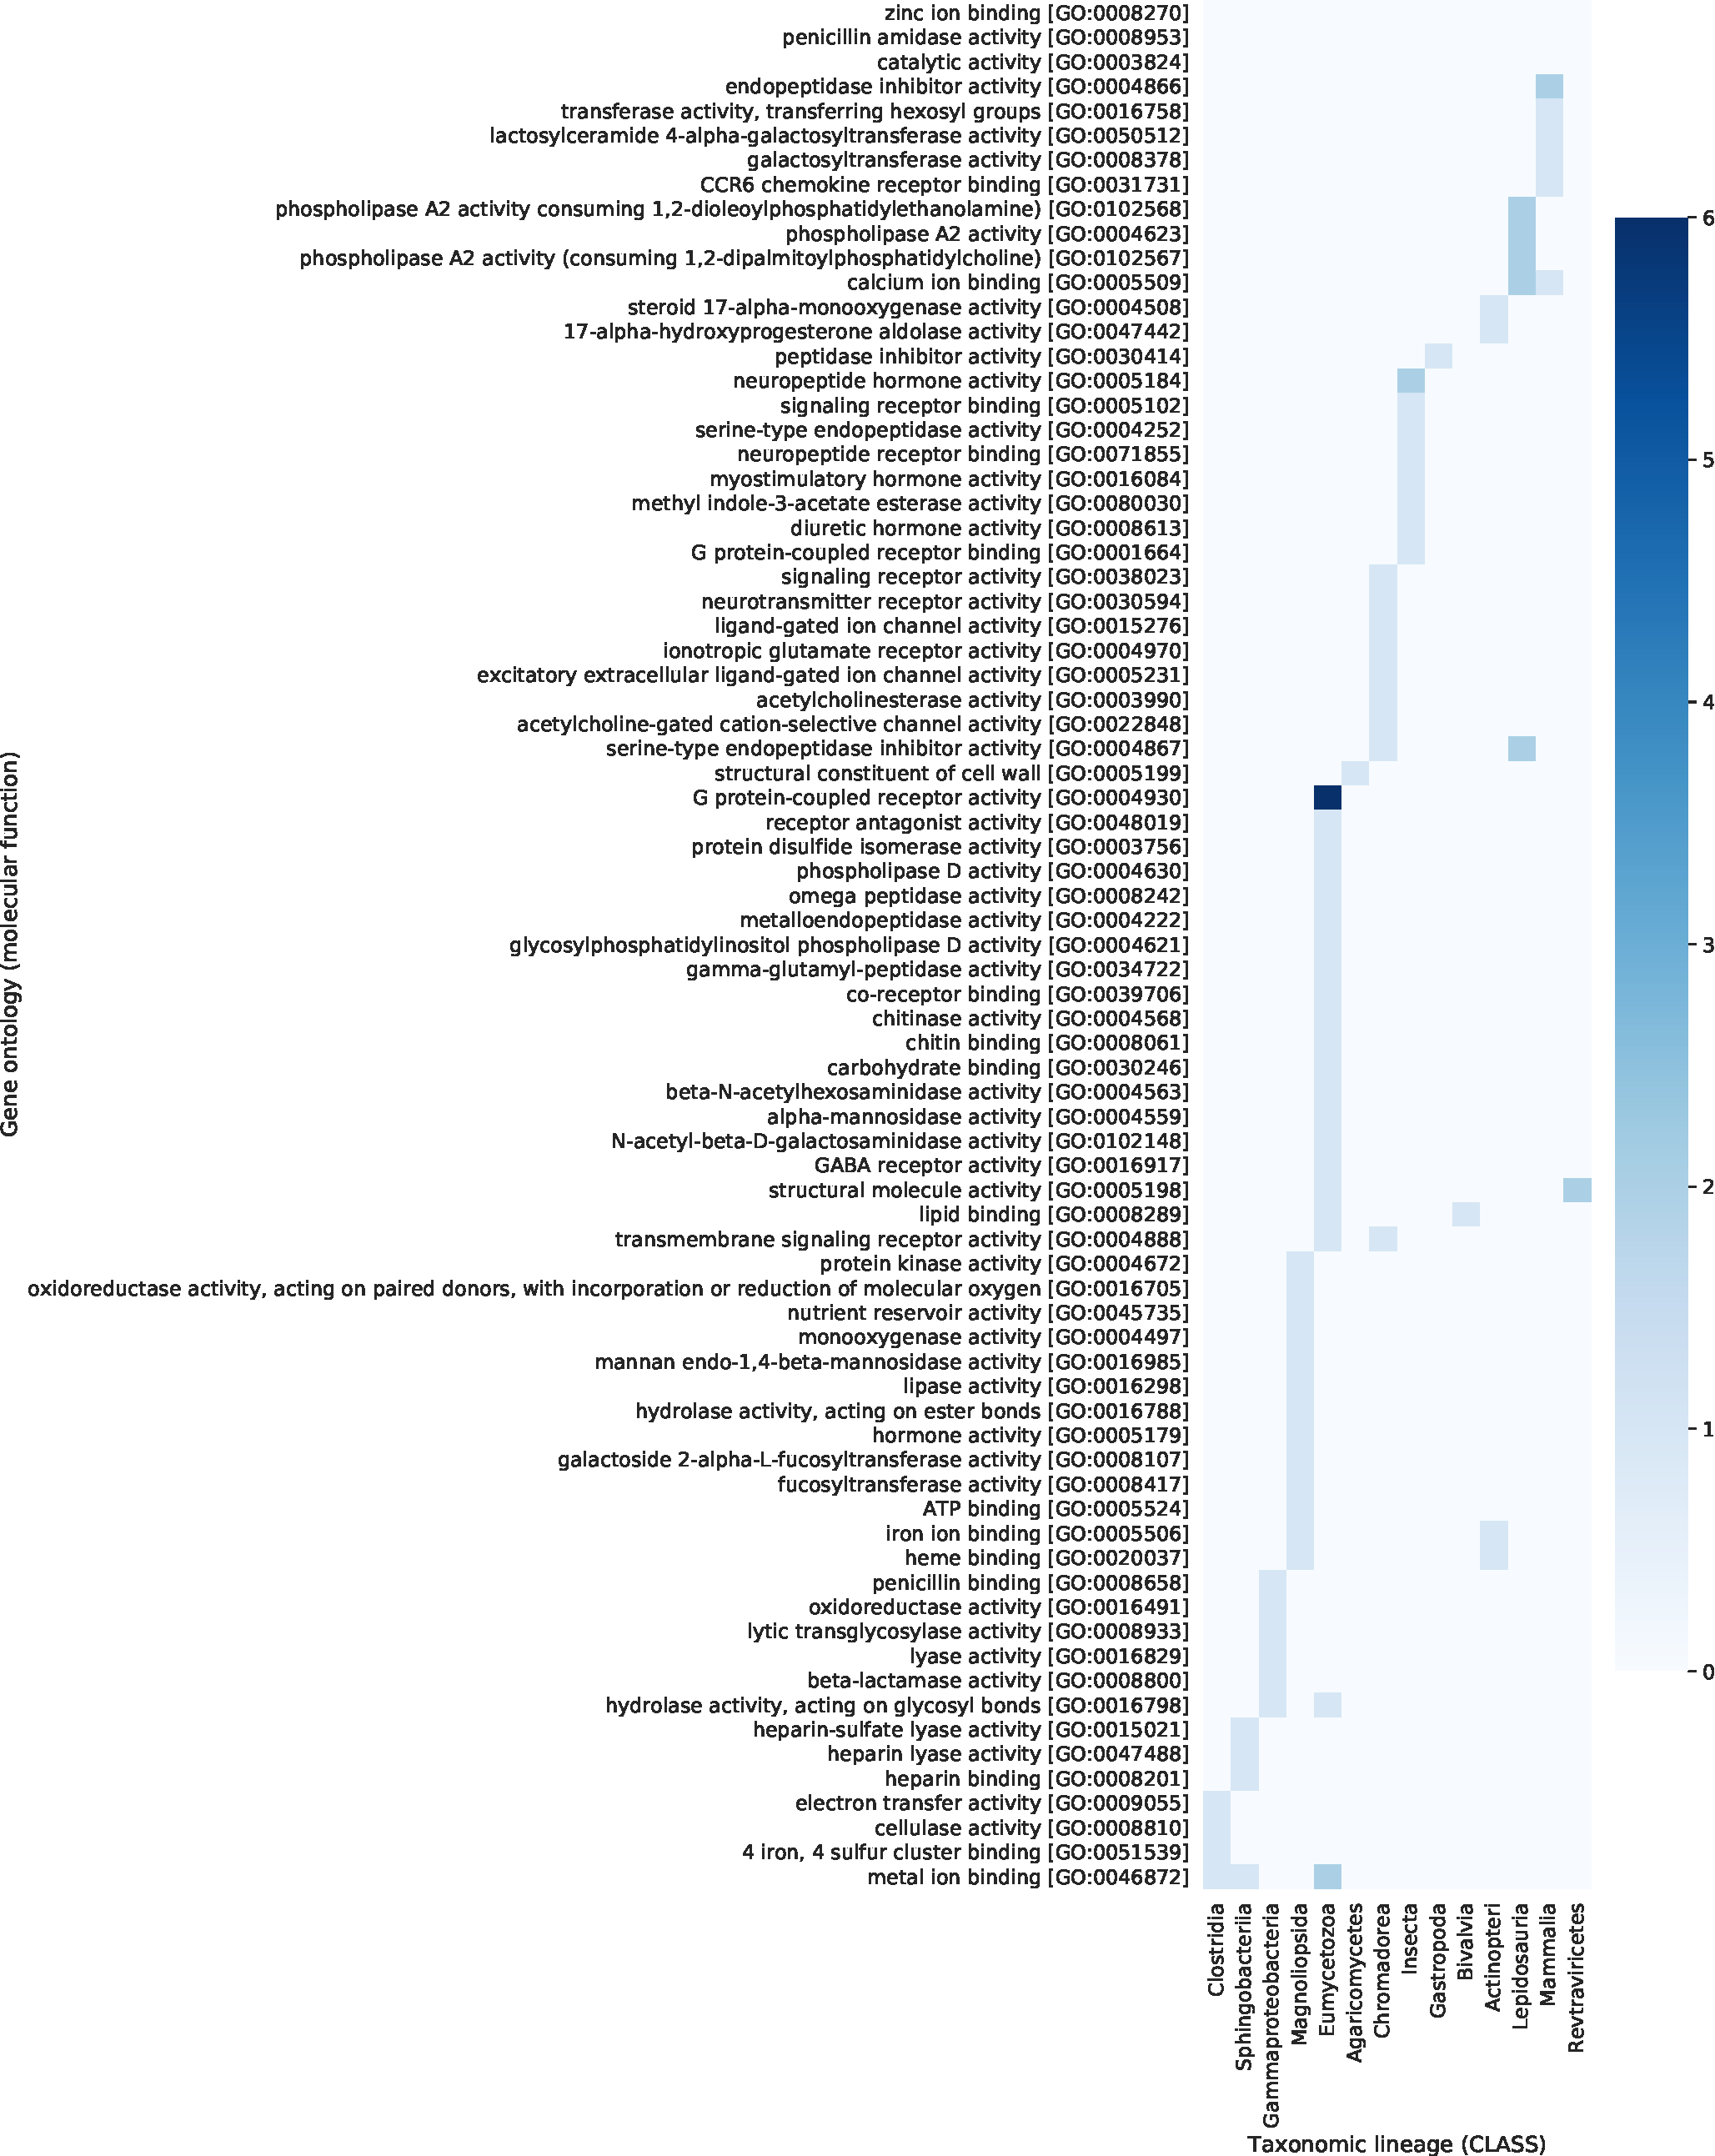
\includegraphics[width=1\textwidth]{appendix/Razor/Figs/toxins_GO_molecular_function.pdf}
\caption[GO annotations (molecular function) for the predicted toxin SPs.]{\textbf{GO annotations (molecular function) for the predicted toxin SPs.} A total of 59 out of 100 predicted sequences had GO terms. The scale bar indicates the frequencies of GO terms for the predicted sequences.

}%the List of Figures because of the *}
\label{fig:appendix_razor_S6}
\end{figure}

\section{Supplementary tables}

\begin{table}[H]
\centering
\caption{Datasets used in this study.}
\begin{tabular}{|l|l|l|}
\hline
\textbf{}   & \textbf{SPs} & \textbf{Non-SPs} \\ \hline
Eukaryotic\textsuperscript{a} & 1,694         & 13,237            \\ \hline
Toxin\textsuperscript{a}      & 261          &                  \\ \hline
Independent test set & \begin{tabular}[c]{@{}l@{}}214\\ (47 Toxin SPs, 194 Non-toxin SPs)\end{tabular} & 52,249 \\ \hline
\end{tabular}

\label{tab:razor_datasets}
\textsuperscript{a}Sequences were retrieved from the SignalP 5.0 training set and the animal toxin annotation program of UniProt and were clustered at 70\% identity using CD-HIT.
\end{table}

\begin{table}[]
\centering
\caption[Feature selection for building the toxin classifier using five-fold cross-validations.]{Feature selection for building the toxin classifier using five-fold cross-validations. Boldface denotes the maximum MCC score.}
\begin{tabular}{|l|l|l|}
\hline
\textbf{N-terminal lengths} & \textbf{MCC scores} & \textbf{Features}                                                                        \\ \hline
15                          & 0.727               & \begin{tabular}[c]{@{}l@{}}Hydrophobicity, SWI, \\ Flexibility, Helix, Turn\end{tabular} \\ \hline
16 & 0.731 & \begin{tabular}[c]{@{}l@{}}Hydrophobicity, SWI, \\ Flexibility, Turn,\\  Isoelectric point\end{tabular} \\ \hline
17                          & 0.716               & \begin{tabular}[c]{@{}l@{}}Hydrophobicity, SWI, \\ Helix, Turn\end{tabular}              \\ \hline
18                          & 0.726               & \begin{tabular}[c]{@{}l@{}}Hydrophobicity, SWI, \\ Isoelectric Point\end{tabular}        \\ \hline
19                          & 0.727               & \begin{tabular}[c]{@{}l@{}}Hydrophobicity, SWI, \\ Turn, Isoelectric Point\end{tabular}  \\ \hline
20                          & 0.727               & \begin{tabular}[c]{@{}l@{}}SWI, Flexibility, Helix, \\ Turn\end{tabular}                 \\ \hline
21                          & 0.718               & \begin{tabular}[c]{@{}l@{}}Hydrophobicity, SWI,\\  Flexibility\end{tabular}              \\ \hline
22                          & 0.717               & \begin{tabular}[c]{@{}l@{}}Hydrophobicity, SWI, \\ Isoelectric Point\end{tabular}        \\ \hline
\textbf{23}                          & \textbf{0.741}               & \begin{tabular}[c]{@{}l@{}}\textbf{Hydrophobicity, SWI,} \\ \textbf{Flexibility, Turn}\end{tabular}        \\ \hline
24                          & 0.715               & Hydrophobicity, SWI                                                                      \\ \hline
25                          & 0.718               & \begin{tabular}[c]{@{}l@{}}Hydrophobicity, Flexibility, \\ Turn\end{tabular}             \\ \hline
26                          & 0.701               & \begin{tabular}[c]{@{}l@{}}Hydrophobicity, SWI,\\  Helix, Isoelectric Point\end{tabular} \\ \hline
27 & 0.716 & \begin{tabular}[c]{@{}l@{}}Hydrophobicity, SWI, \\ Flexibility, Isoelectric Point\end{tabular}          \\ \hline
28                          & 0.712               & \begin{tabular}[c]{@{}l@{}}Hydrophobicity, SWI, \\ Turn\end{tabular}                     \\ \hline
\end{tabular}

\label{tab:razor_feature_selection}
\end{table}

\begin{table}[]
\centering
\caption[Benchmarking of eukaryotic SP prediction using an independent test set (toxin SPs=287, Non-SPs=52,055).]{Benchmarking of eukaryotic SP prediction using an independent test set (toxin SPs=287, Non-SPs=52,055). Boldface denotes the maximum MCC score.
}
\begin{tabular}{|l|l|l|l|l|}
\hline
\textbf{} & \textbf{SignalP 5.0} & \textbf{DeepSig} & \textbf{SignalP 4.1} & \textbf{Razor} \\ \hline
MCC       & \textbf{0.571}                & 0.537            & 0.511                & 0.405          \\ \hline
\end{tabular}

\label{tab:razor_benchmark_independent_test_set_mcc}
\end{table}


% Please add the following required packages to your document preamble:
% \usepackage{multirow}
\begin{table}[]
\centering
\caption[Benchmarking of the cleavage site prediction for eukaryotic SPs using an independent test set (SPs=287, Non-SPs=52,055).]{Benchmarking of the cleavage site prediction for eukaryotic SPs using an independent test set (SPs=287, Non-SPs=52,055). Boldface denotes the highest scores.
}
\begin{tabular}{|l|l|l|l|l|}
\hline
\multirow{2}{*}{\textbf{Tools}} & \multicolumn{4}{l|}{\textbf{Distance around the cleavage sites}} \\ \cline{2-5} 
            & 0              & $\pm1$              & $\pm2$              & $\pm3$              \\ \hline
\multicolumn{5}{|c|}{Cleavage site precision}                                   \\ \hline
SignalP 5.0 & \textbf{0.287} & \textbf{0.306} & \textbf{0.33}  & \textbf{0.34}  \\ \hline
SignalP 4.1 & 0.229          & 0.247          & 0.26           & 0.266          \\ \hline
Razor       & 0.136          & 0.15           & 0.164          & 0.171          \\ \hline
DeepSig     & 0.237          & 0.261          & 0.301          & 0.31           \\ \hline
\multicolumn{5}{|c|}{Cleavage site recall}                                      \\ \hline
SignalP 5.0 & \textbf{0.704} & \textbf{0.749} & \textbf{0.808} & \textbf{0.833} \\ \hline
SignalP 4.1 & 0.693          & 0.746          & 0.787          & 0.805          \\ \hline
DeepSig     & 0.53           & 0.582          & 0.672          & 0.693          \\ \hline
Razor       & 0.596          & 0.655          & 0.718          & 0.746          \\ \hline
\end{tabular}

\label{tab:razor_benchmark_independent_test_set_precision_recall}
\end{table}


\begin{table}[]
\centering
\caption[Benchmarking of toxin SP prediction using an independent test set (toxin SPs=47, Non-toxin SPs=52,055).]{Benchmarking of toxin SP prediction using an independent test set (toxin SPs=47, Non-toxin SPs=52,055). Boldface denotes the maximum MCC score.
}
\begin{tabular}{|l|l|l|l|l|}
\hline
\textbf{} & \textbf{SignalP 5.0} & \textbf{DeepSig} & \textbf{SignalP 4.1} & \textbf{Razor} \\ \hline
MCC       & 0.301                & 0.300            & 0.260                & \textbf{0.611}          \\ \hline
\end{tabular}

\label{tab:razor_benchmark_independent_test_set_toxin_mcc}
\end{table}

% Please add the following required packages to your document preamble:
% \usepackage{multirow}
\begin{table}[]
\centering
\caption[Benchmarking of the cleavage site prediction for toxin SPs using an independent test set (toxin SPs=47, Non-toxin SPs=52,055).]{Benchmarking of the cleavage site prediction for toxin SPs using an independent test set (toxin SPs=47, Non-toxin SPs=52,055). Boldface denotes the highest scores.
}
\begin{tabular}{|l|l|l|l|l|}
\hline
\multirow{2}{*}{\textbf{Tools}} & \multicolumn{4}{l|}{\textbf{Distance around the cleavage sites}} \\ \cline{2-5} 
            & 0              & $\pm1$              & $\pm2$              & $\pm3$      \\ \hline
\multicolumn{5}{|c|}{Cleavage site precision}                                   \\ \hline
SignalP 5.0 & 0.094          & N/A            & N/A            & 0.34           \\ \hline
SignalP 4.1 & 0.065          & 0.068          & 0.07           & 0.266          \\ \hline
Razor       & \textbf{0.355} & \textbf{0.373} & \textbf{0.382} & \textbf{0.171} \\ \hline
DeepSig     & 0.073          & 0.077          & 0.097          & 0.31           \\ \hline
\multicolumn{5}{|c|}{Cleavage site recall}                                      \\ \hline
SignalP 5.0 & \textbf{0.979} & \textbf{N/A}   & \textbf{N/A}   & \textbf{0.833} \\ \hline
SignalP 4.1 & 0.915          & 0.957          & 0.979          & 0.805          \\ \hline
DeepSig     & 0.702          & 0.745          & 0.936          & 0.693          \\ \hline
Razor       & 0.830          & 0.872          & 0.894          & 0.746          \\ \hline
\end{tabular}

\label{tab:razor_benchmark_independent_test_set_toxin_precision_recall}
\end{table}